\documentclass{article}

\usepackage[utf8]{inputenc}
\usepackage[danish]{babel}
\usepackage{float}
\usepackage{fancyhdr}
\usepackage{amsmath}
\usepackage{color}
\usepackage{listings}
\usepackage{graphicx}
\usepackage{pdfpages}
\usepackage{booktabs}
%\usepackage{enumitem}
\usepackage[a4paper, top = 1in, bottom = 1in, left=1in,right=1in]{geometry}

\title{Tællende Aktivitet 2}
\author{Peter Heilbo Ratgen \\ perat17}
\date{\today}

\begin{document}
\maketitle

\section{Opgave 1}
\subsection{Deskriptiv analyse}
En deskriptiv analyse af udgifterne til behandling af patienter 
\textsc{Treatcost}. 
\begin{figure}[h]
  \centering
  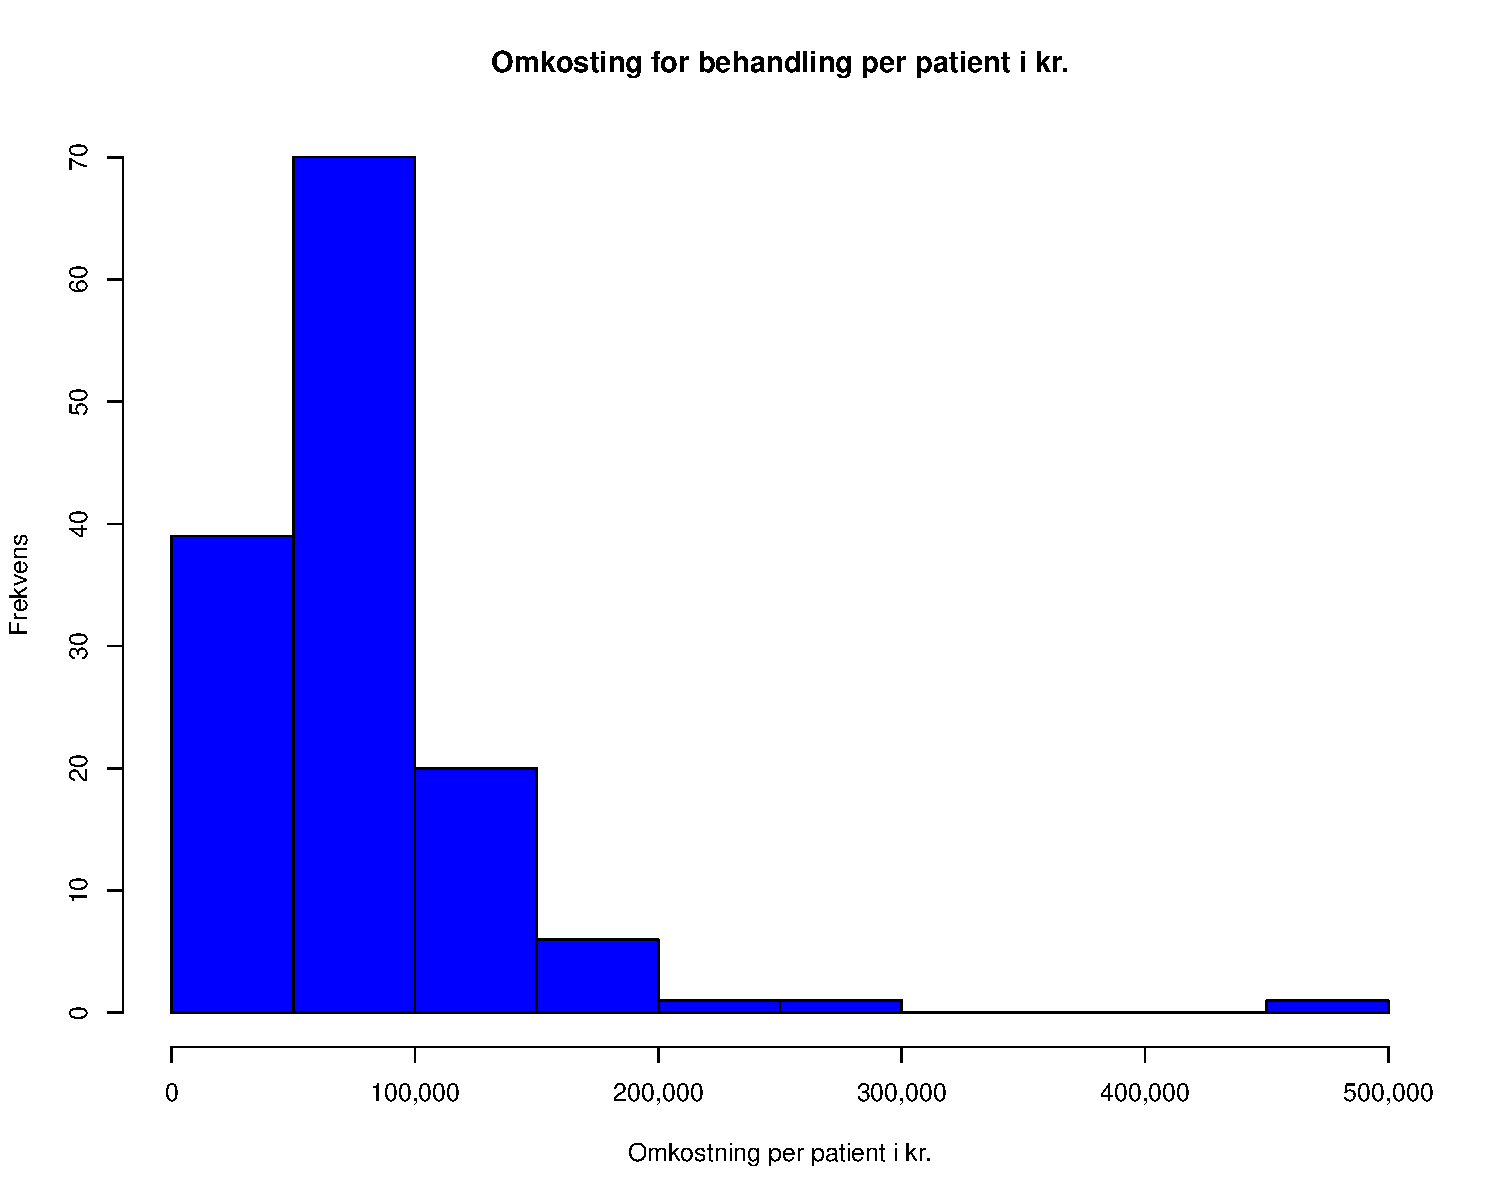
\includegraphics[width=0.6\textwidth]{./treatcost.pdf}
  \caption{Histogram af omkostningen for at behandle patienter}
\end{figure}



% Histogram
% Summering af nøgletal
% Modus
% Standardafvigelse


% Konklusion

\section*{Opgave 2}

% Konklusion

\section*{Opgave 3}

% Konklusion

\section*{Opgave 4}

% Konklusion

\section*{Opgave 5}

% Konklusion

\end{document}

